\newpage 
\section{Kiến trúc hệ thống}
\begin{figure}[H]
	\centering
	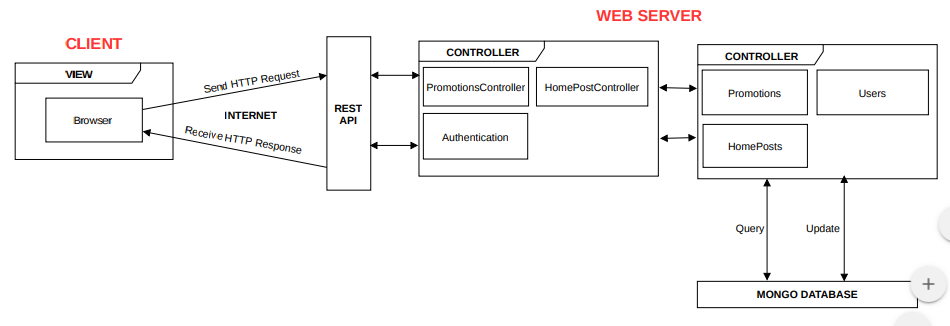
\includegraphics[width=14cm]{Image/ar.png}
	\vspace{0.5cm}
	\caption{Kiến trúc hệ thống}
\end{figure}

Mẫu thiết kế được dùng cho hệ thống chia sẻ nhà DiamondStay là MCV (Model-Controller-View) dành cho web. Mô hình này khá phổ biến cho các ứng dụng web. \\
Controller bao gồm các các controller sau:
\begin{itemize}
    \item HomePostController: Điều khiển các hoạt động liên quan đến đăng bài, duyệt bài.
    \item PromotionsController: Điều khiển các hoạt động liên quan đến khuyến mãi như tạo khuyến mại, xóa khuyến mãi, chỉnh sửa khuyến mãi,...
    \item Authentication: Điều khiển các hoạt động liên quan đến xác thực người dùng.
    \item BookingController: Điều khiển các hoạt động liên quan đến tìm kiếm, đặt phòng.
    \item MessageController: Điều khiển các hoạt động liên quan đế tin nhắn.
\end{itemize}

Model bao gồm các các model sau:
\begin{itemize}
    \item HomePost: Định nghĩa và quản lí truy vấn, cập nhật, xóa dữ liệu về các tin đăng cho thuê homestay.
    \item Users: Định nghĩa và quản lí truy vấn, cập nhật, xóa dữ liệu về thông tin người dùng.
    \item Promotions: Định nghĩa và quản lí truy vấn, cập nhật, xóa dữ liệu về khuyến mãi.
    \item Message: Định nghĩa và quản lí truy vấn, cập nhật, xóa dữ liệu tin nhắn giữa các người dùng.
\end{itemize}